\documentclass[20pt]{article}

\usepackage[english]{babel}
\usepackage[utf8x]{inputenc}
% \usepackage{amsmath}
\usepackage{graphicx}
\usepackage[margin=0.8in]{geometry}

\title{AS205:Ocean Dynamics(Assignment 5)}
\author{Parag Shende}

\begin{document}
\maketitle
\hrule

\section*{Introduction}

We describe the seasonal mean stratification in the Bay of Bengal and Arabian sea. 

\section*{Datasets}

The datasets used in this analysis is as follows:

\begin{itemize}
    \item \textbf{Density} : World Ocean Atlas(WOA18)
\end{itemize}

\section*{Methodology}

The datasets are choosen for the domain of $40^{\circ} E$ to $100^{\circ}E$ and $0^{\circ} N$ to $25^{\circ} N$. This covers the
North Indian ocean. We then calculate the seasonal mean with the following seasons:

The density data was chosen for the transect at $70^{\circ} E$ for the Arabian sea and $88^{\circ} E$ for the Bay of Bengal. Both the 
transect extend from $10^{\circ} N$ to $20^{\circ} N$ .We choose seasonal means were as follows 

\begin{itemize}
    \item \textbf{Summer Monsoon} : June, July, August, September(JJAS)
    \item \textbf{Winter Monsoon} : December, January, February(DJF)
\end{itemize}

The stratification is measured by the Brunt-Vaisale frequency calculated as:

\begin{center}
   $N^{2} = - \frac{g}{\rho_{0}} \frac{\partial\rho}{\partial z}$
\end{center}

where,

$\rho_{0}$ is the reference density. 

$\rho$ is the density of the water at different levels. 




\section*{Bay of Bengal}

\begin{figure}
    \centering
    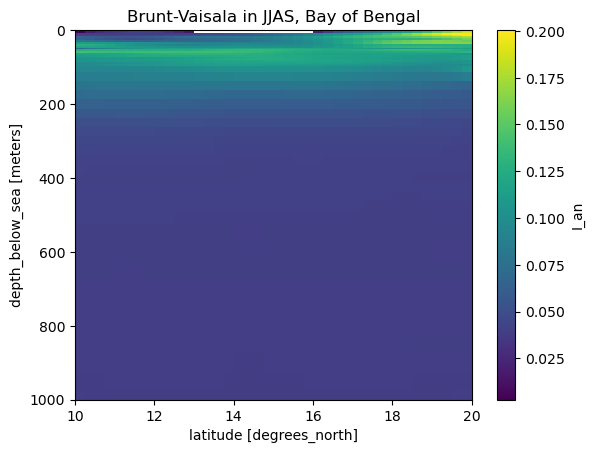
\includegraphics[width=0.6\textwidth]{n_summer_bob.png}
    \caption{stratification of Bay of Bengal in summer ($s^{-1}$)}
\end{figure}

\begin{figure}
    \centering
    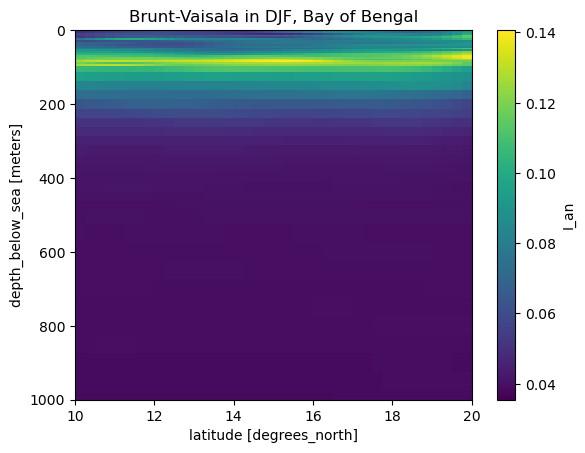
\includegraphics[width=0.6\textwidth]{n_winter_bob.png}
    \caption{stratification of Bay of Bengal in winter ($s^{-1}$)}
\end{figure}

\begin{itemize}
    \item The seasonal mean stratification for the Bay of Bengal is plotted in Figure 1(Summer) and Figure 2(Winter).
    \item We observe the pycnocline is deeper in the post-monsoon DJF period(around 100m) as compared to the pre-monsoon period(around 30m).
    \item Overall the stratification is higher in the post-monsoon period in the bay. 
\end{itemize}

\section*{Arabian Sea}

\begin{figure}
    \centering
    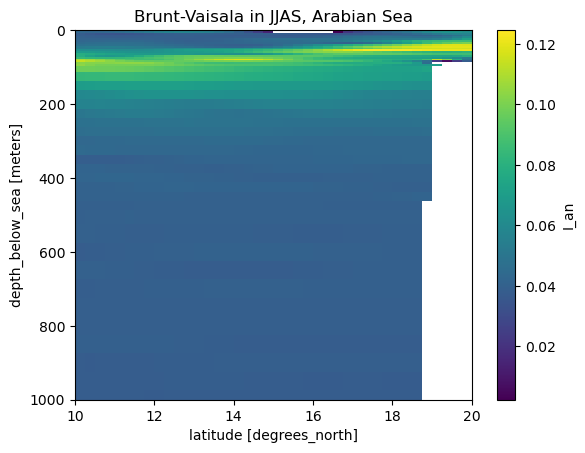
\includegraphics[width=0.6\textwidth]{n_summer_as.png}
    \caption{stratification of Arabian sea in summer ($s^{-1}$)}
\end{figure}

\begin{figure}
    \centering
    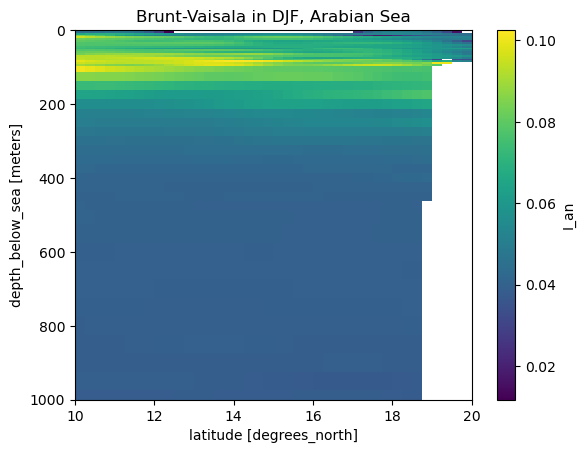
\includegraphics[width=0.6\textwidth]{n_winter_as.png}
    \caption{stratification of Arabian sea in winter ($s^{-1}$)}
\end{figure}

\begin{itemize}
    \item The seasonal mean stratification for the Arabian sea is plotted in Figure 3(Summer) and Figure 2(Winter).
    \item The stratification is nearly constant in both the periods.
    \item The pycnocline in both the periods is around 100m. 
\end{itemize}

\end{document}